\documentclass[11pt]{article}
\usepackage{actstyle}
\settitle{ACT Reading: Full-Length Practice Section}{Volume 2 --- 36 Questions, 40 Minutes}

\begin{document}
\maketitleblock

\begin{abstract}
This is a complete, original practice section built to Enhanced ACT Reading specifications: four passage units with nine questions each, 36 questions in 40 minutes. It uses the format combination of two single passages, one paired set, and one passage with a figure, so every passage format appears. The four units cover the four content areas---Literary Narrative, Social Science, Humanities, and Natural Science---and the questions follow ACT's reporting-category proportions (about 47\% Key Ideas \& Details, 31\% Craft \& Structure, and 22\% Integration of Knowledge \& Ideas). The answer key on the final pages gives each answer, the textual evidence behind it, and the rule from Volume~1 it tests, along with a diagnostic table by category.
\end{abstract}

\scoreline{\textbf{Time:} 40 minutes}

\begin{notebox}
\small
\textbf{Directions.} This section contains four passage units, each followed by nine questions. Read each passage, then choose the best answer to each question and write its letter in the blank beside the question number. You may refer to the passages as often as necessary. There is no penalty for guessing, so answer every question.\par\vspace{3pt}
\textbf{Clock checkpoints.} Unit I by 10:00 $\cdot$ Unit II by 20:00 $\cdot$ Unit III by 30:00 $\cdot$ Unit IV by 40:00.\par\vspace{3pt}
\textbf{Note.} All passages are original and were written for this section. The people, places, and data in Passages II and IV are fictional or illustrative; historical figures and quotations in Passage III are real.
\end{notebox}

% =====================================================================
\clearpage
\passagehead{PASSAGE I}{LITERARY NARRATIVE}{This passage is an original short story. The narrator recalls a summer spent assisting a parent who tuned pianos.}
\begin{passage}
The summer I turned sixteen, my father decided I was old enough to carry his case. It was a narrow leather thing, scuffed pale at the corners, and it held everything he believed a piano might need: tuning hammer, rubber mutes, a felt strip as long as my arm, a tin of graphite, and a tuning fork he never once used in my presence but would not leave home without. \linelabel{p1case}``In case the world goes out of tune,'' he said, when I asked, and I rolled my eyes in the way that sixteen-year-olds are permitted to.

I had imagined the job would be about music. It was mostly about waiting. We waited in front halls while dogs were shut in back rooms. We waited while lids were cleared of photographs and plants and, once, an entire collection of ceramic owls. And when the piano was finally bare, my father waited again---sitting on the bench with his hands in his lap, not touching anything, just looking at the instrument as if it had something to tell him and he did not want to interrupt.

\linelabel{p1start}``Why don't you just start?'' I asked him at the third house.

``I did,'' he said.\linelabel{p1did}

The owners were always the same and never the same. There was the retired dentist whose baby grand had been his late wife's and who stood in the doorway the whole hour as if guarding it. There was a family whose upright had been dragged across three states and whose six-year-old played the same four bars of a march so many times that I began to hear them in my sleep. There was Mrs.~Okafor, who apologized for the state of her spinet before we had even set down the case, and then apologized for apologizing.

\linelabel{p1ask}My father spoke very little to any of them. He asked how long they had owned the piano, who played it, and whether it lived near a window or a radiator. Then he listened---to the piano, I assumed. He would strike a key, hold it, and tilt his head, and the room would go so quiet that I could hear the refrigerator two rooms away. Then he would set the hammer on a pin and turn it a distance too small for me to see.

\linelabel{p1ok}It was at Mrs.~Okafor's that I began to understand what I had been watching. Halfway through the job, she brought us lemonade and stayed, hovering by the bookcase, and my father---who had said perhaps twenty words that whole morning---asked her whether she played. Not much anymore, she said. Her daughter had taken lessons; the daughter lived in Lagos now, and the piano was mostly furniture. My father nodded and went back to work. But a few minutes later, without looking up, he asked what her daughter used to play, and when she named a piece, he played the opening of it, softly, testing the middle octaves. \linelabel{p1laugh}Mrs.~Okafor laughed and put her hand over her mouth. Then she sat down in the armchair by the window and did not apologize again for the rest of the hour.\linelabel{p1okend}

\linelabel{p1car}In the car I said, ``You didn't need to play that. The middle was already fine.''

``The piano was fine,'' he agreed.\linelabel{p1fine}

I spent the rest of the summer trying to hear what he heard. I learned to set a mute and to recognize the slow wobble that meant two strings were nearly but not quite agreeing. I never learned to hear what he heard in the rooms themselves: the dentist's grief, the family's exhaustion, the particular note of loneliness that made a person apologize to strangers for her furniture. My father, I think, would have said there was no difference. A piano under strain and a person under strain both pull slightly away from \linelabel{p1true}true, and the work in both cases is the same: patience, attention, and a turn of the hand so small that no one watching would call it work at all.

\linelabel{p1now}I carry my own case now, though what is in it has nothing to do with pianos. The tuning fork is in there. I have never used it. I don't intend to leave home without it.\linelabel{p1end}
\end{passage}

\Q{KID}{B}{Central idea (R3)}{The passage builds to the narrator's realization at Mrs.~Okafor's (\Line{p1ok}) that the father tunes people as well as pianos (\lines{p1true}{p1end}). A is contradicted: the narrator's case ``has nothing to do with pianos.'' C is too narrow; D invents a change in the father.}
{Which of the following best describes the main idea of the passage?}
{A teenager reluctantly learns a trade and eventually decides to make it a career.}
{A narrator recalls gradually recognizing that the father's work involved attending to people as closely as to instruments.}
{A father teaches his child the technical steps of piano tuning over one summer.}
{A narrator describes how a series of customers changed the father's attitude toward his job.}

\Q{KID}{D}{Stated detail, EXCEPT (R1)}{Paragraph 1 lists hammer, mutes, felt strip, graphite, and tuning fork. No metronome is mentioned.}
{According to the passage, the father's case contained all of the following EXCEPT:}
{a tin of graphite.}{rubber mutes.}{a felt strip.}{a metronome.}

\Q{CS}{A}{Function of a detail (R7)}{The father's ``I did'' (\Line{p1did}) shows that his silent looking---which the narrator took for waiting---was already part of the job.}
{The exchange in \lines{p1start}{p1did} primarily serves to:}
{show that the father considered his silent observation to be part of the work.}
{suggest that the father was annoyed by the narrator's impatience.}
{reveal that the narrator had confused one house with another.}
{indicate that the father had tuned the piano before the narrator arrived.}

\Q{KID}{B}{Inference (R2)}{She laughs and covers her mouth right after he plays ``the opening'' of the piece her daughter used to play---a moment of recognition. Nothing suggests embarrassment (A) or judgment of his playing (C).}
{It can reasonably be inferred that Mrs.~Okafor laughed and put her hand over her mouth (\Line{p1laugh}) because she:}
{was embarrassed that her piano was so badly out of tune.}
{recognized the music as the piece her daughter used to play.}
{thought the father's playing was technically clumsy.}
{was surprised that the father had stopped working to rest.}

\Q{KID}{A}{Stated detail (R1)}{``He asked how long they had owned the piano, who played it, and whether it lived near a window or a radiator'' (\Line{p1ask}).}
{According to the passage, the questions the father usually asked owners concerned:}
{the piano's history, who played it, and where it stood in the house.}
{the owners' musical training and favorite composers.}
{the price the owners had paid for the piano.}
{whether the owners planned to sell the piano.}

\Q{CS}{D}{Word in context (R5)}{Strings ``nearly but not quite agreeing'' pull away from correct pitch; ``true'' here means proper alignment, as in a wheel or a note being true. A and D are the common-meaning traps.}
{As it is used in \Line{p1true}, the word \emph{true} most nearly means:}
{honest.}{loyal.}{factual.}{proper alignment.}

\Q{CS}{B}{Point of view (R8)}{``I carry my own case now'' (\Line{p1now}) and ``The summer I turned sixteen'' place the narrator as an adult looking back.}
{The passage is told from the point of view of a narrator who is:}
{a teenager describing events as they happen.}
{an adult looking back on an experience from adolescence.}
{an outside observer who reports the father's private thoughts.}
{the father, remembering his first summer as a tuner.}

\Q{KID}{C}{Inference (R2)}{``The \emph{piano} was fine'' (\Line{p1fine}) agrees the instrument needed nothing while implying the playing served someone else---Mrs.~Okafor.}
{The father's reply in \Line{p1fine} most strongly suggests that he:}
{believed the narrator had misheard the middle octaves.}
{had played the piece mainly to test the narrator's ear.}
{agreed the piano needed no more work but had played for a different reason.}
{regretted having taken longer than necessary on the job.}

\Q{IKI}{C}{Claims and evidence (R9)}{Carrying the father's tuning fork and refusing to leave home without it echoes the father's habit---evidence the narrator came to value his way of working. A shows early dismissiveness; B and D describe the job, not the narrator's view of it.}
{Which quotation from the passage best supports the claim that the narrator came to value the father's way of working?}
{``I rolled my eyes in the way that sixteen-year-olds are permitted to''}
{``It was mostly about waiting.''}
{``The tuning fork is in there. I have never used it. I don't intend to leave home without it.''}
{``the room would go so quiet that I could hear the refrigerator two rooms away''}

% =====================================================================
\clearpage
\passagehead{PASSAGE II}{SOCIAL SCIENCE}{Passage A is written from the perspective of a rural school superintendent. Passage B is written from the perspective of an education economist. Both passages are original.}
\subpassage{Passage A}
\begin{passage}
When our district moved to a four-day week six years ago, the decision was not ideological. \linelabel{p2arith}It was arithmetic. We serve a county larger than some states, our buses travel more than a thousand miles a day, and for three straight years we had ended spring with teaching positions we could not fill. Closing on Fridays trimmed transportation, utility, and substitute costs. The savings were modest---families who expected a windfall were disappointed---but they were real, and in a budget like ours, modest is not trivial.

\linelabel{p2a2}The larger effect was one no spreadsheet predicted. The first year after the switch, applications for open positions nearly doubled. Teachers told us, sometimes in their interviews, that a three-day weekend was worth more to them than the raise we could not afford to offer. Our attrition fell. For a rural district, a stable faculty is not a perk; it is the precondition for everything else.

\linelabel{p2a3}Critics point to studies showing small declines in test scores in some four-day districts, and I take those studies seriously. But averages conceal choices. Districts that simply compressed five days of instruction into four, adding forty minutes to the end of an already long day, have reason to worry. Districts that rebuilt the schedule---protecting morning time for core subjects, using Fridays for tutoring and enrichment for students who want it---tell a different story. The four-day week is not a reform in itself. It is a frame, and \linelabel{p2frame}what matters is what a district builds inside it.\linelabel{p2aend}
\end{passage}
\subpassage{Passage B}
\begin{passage}[cont]
\linelabel{p2b1}The case for the four-day school week is usually made by the adults who work in schools, and it is easy to see why. A three-day weekend is an attractive benefit, and in places where recruiting teachers is a \linelabel{p2per}perennial crisis, it may be the only benefit a district can offer. But a school calendar is not only a staffing policy. It is also, for millions of families, a child-care arrangement, a meal program, and the most reliable source of structure in a child's week.

\linelabel{p2b2}Consider what happens on the fifth day. For a family with two working parents, Friday becomes a problem to be solved---by a grandparent, an older sibling, a paid program, or, too often, by no one. The district's savings on buses and heating do not vanish; they are partly transferred to households, and they fall hardest on the households least able to absorb them. Students who relied on school breakfast and lunch lose a fifth of those meals.\linelabel{p2b2end}

Nor is the academic picture as reassuring as advocates suggest. The research is still young, and results vary, but the more careful recent studies tend to find that, on average, students in four-day districts learn somewhat less over time than similar students in five-day districts---and that the gap is larger where instructional hours were cut. Some districts have done better than average, and I would like to know how. \linelabel{p2last}But a policy should be judged by what it typically produces, not by what its best practitioners achieve.
\end{passage}

{\small\itshape Questions 10--12 ask about Passage A. Questions 13--15 ask about Passage B. Questions 16--18 ask about both passages.}

\Q{CS}{A}{Word choice / function (R6)}{Contrasting ``not ideological'' with ``arithmetic'' stresses that the decision came from budget and staffing numbers. D is never stated.}
{In Passage A, the statement ``It was arithmetic'' (\Line{p2arith}) primarily serves to:}
{emphasize that the district's decision was driven by practical constraints rather than beliefs.}
{suggest that the decision was made mainly by the district's math teachers.}
{admit that the district miscalculated the savings.}
{criticize districts that adopted the policy for ideological reasons.}

\Q{KID}{B}{Stated detail (R1)}{``The larger effect was one no spreadsheet predicted. \dots\ applications for open positions nearly doubled'' (\Line{p2a2}). Cost savings (A) were the expected effect.}
{According to Passage A, which outcome of the four-day week was unexpected?}
{Lower transportation costs}
{A sharp rise in applications for teaching positions}
{Disappointment among some families}
{Higher test scores}

\Q{KID}{D}{Relationships (R4)}{Paragraph 3 contrasts districts that ``simply compressed'' instruction with those that ``rebuilt the schedule''---the difference is how instruction was structured.}
{The author of Passage A suggests that the difference between four-day districts that saw test-score declines and those that did not is mainly related to:}
{the size of each district's budget.}
{whether teachers received raises.}
{how far students traveled to school.}
{how each district structured instruction within the four-day week.}

\Q{KID}{A}{Paragraph main idea (R3)}{Paragraph 2 of Passage B (\lines{p2b2}{p2b2end}): savings are ``partly transferred to households''---child care and meals become families' burden. B and C are details; D contradicts nothing but is never argued.}
{The main point of the second paragraph of Passage B is that the four-day week:}
{shifts some costs and burdens from the district onto families.}
{relies most heavily on grandparents for Friday child care.}
{requires schools to expand meal programs to Fridays.}
{saves districts more money than its advocates admit.}

\Q{CS}{D}{Word in context (R5)}{A recruiting crisis that keeps returning year after year is \emph{recurring}. ``Seasonal'' (A) is the trap from the botanical sense of \emph{perennial}.}
{As it is used in \Line{p2per}, the word \emph{perennial} most nearly means:}
{seasonal.}{growing.}{occasional.}{recurring.}

\Q{IKI}{B}{Evaluating reasoning (R9)}{\Line{p2last}: a policy ``should be judged by what it typically produces, not by what its best practitioners achieve.''}
{In the last sentence of Passage B, the author reasons that a policy should be evaluated according to:}
{the results achieved by the most successful districts.}
{its typical outcomes rather than its best cases.}
{the preferences of the teachers it affects.}
{how recently it was adopted.}

\Q{IKI}{C}{Synthesis: agreement (R10)}{A: applications doubled. B: the benefit is attractive and ``may be the only benefit a district can offer.'' Both accept the recruiting advantage. A and B are rejected by Passage B; D appears only in Passage A.}
{Both authors would most likely agree that the four-day week:}
{reliably improves student achievement.}
{produces substantial savings for districts.}
{can help districts attract teachers.}
{should include tutoring on Fridays.}

\Q{IKI}{C}{Synthesis: response (R10)}{B grants that ``Some districts have done better than average'' but insists policy be judged by typical results---a direct answer to A's ``what matters is what a district builds inside it'' (\Line{p2frame}).}
{How would the author of Passage B most likely respond to the claim in Passage A that ``what matters is what a district builds inside it''?}
{By agreeing that outcomes depend entirely on district choices, so the policy should be adopted widely}
{By arguing that test scores do not measure student learning}
{By granting that some districts do better than average while insisting that the policy be judged by its typical results}
{By pointing out that rural districts cannot afford Friday tutoring}

\Q{IKI}{A}{Synthesis: contrast (R10)}{B's second paragraph is devoted to child care, meals, and household costs on the fifth day; A focuses on budget, staffing, and schedule design.}
{Compared with Passage A, Passage B places greater emphasis on the four-day week's:}
{effects on families outside of school hours.}
{effects on teacher recruitment.}
{strategies for building an effective schedule.}
{personal significance to a district leader.}

% =====================================================================
\clearpage
\passagehead{PASSAGE III}{HUMANITIES}{This passage is an original essay on the history of architectural restoration.}
\begin{passage}
In April 2019, as the spire of Notre-Dame de Paris collapsed into the burning nave, millions of people watched something fall that was, strictly speaking, not medieval. \linelabel{p3spire}The spire had been designed in the 1850s by the architect Eug\`ene Viollet-le-Duc to replace a thirteenth-century predecessor that had been taken down, in poor condition, in the 1780s. Few of the mourners knew this, and I am not sure it would have mattered to them if they had. The spire was part of what Notre-Dame looked like.

Viollet-le-Duc was the most influential restorer of his century, and he was unusually \linelabel{p3cand}candid about what he was doing. ``To restore a building,'' he wrote, ``is not to maintain it, repair it, or rebuild it; it is to reestablish it in a complete state that may never have existed at any given moment.'' For him, a restorer was something like a translator who understood the original author better than the author had understood himself. Where the medieval builders had left a cathedral unfinished, or where later centuries had altered it, the restorer's job was to supply the building the original logic implied. He applied this principle at Notre-Dame, at the walled city of Carcassonne, and at dozens of other sites, and the France that tourists photograph today is in no small part his invention.

Across the Channel, the critic John Ruskin regarded this as vandalism dressed in scholarship. Restoration, he wrote in 1849, ``means the most total destruction which a building can suffer.'' A building's value, for Ruskin, lay not only in its design but in the marks of the particular hands that made it and the particular centuries that weathered it. A carved stone recut by a nineteenth-century mason was not the old stone improved; it was a new stone telling a lie. His advice was blunt: take care of old buildings---prop them, patch their roofs, keep the water out---and when they can no longer be saved, let them go. Ruskin's follower William Morris later founded the Society for the Protection of Ancient Buildings on this principle, and its members cheerfully adopted the nickname ``Anti-Scrape.''

\linelabel{p3p4}I used to think Ruskin was simply right. There is something unsettling about a restoration that erases the evidence of time in order to produce a building more perfect than any that ever stood. But standing in Carcassonne a few years ago---among walls and towers that are, in their present form, largely Viollet-le-Duc's---I found I could not quite summon the outrage I had brought with me. The place was moving. Children ran along the ramparts. Whatever it was, it was not a lie anyone there felt they were being told.\linelabel{p3p4end}

\linelabel{p3p5}The truth, I have come to believe, is that the two men were answering different questions. Ruskin asked what a building \emph{is}: an object, a piece of evidence, a document of the past that, like any document, is falsified by revision. Viollet-le-Duc asked what a building is \emph{for}. A cathedral is not only an artifact but a place where people gather, and a ruin cannot do that. Most modern preservation codes try to split the difference. They encourage repair over replacement, require new work to be distinguishable on close inspection, and demand that every intervention be recorded---\linelabel{p3consc}Ruskin's conscience, in other words, applied to Viollet-le-Duc's ambition.

\linelabel{p3p6}The decision to rebuild Notre-Dame's spire exactly as Viollet-le-Duc designed it, rather than replace it with something new, was therefore a stranger choice than it first appeared. It was a faithful copy of an object that was itself a confident invention. I don't think that makes it wrong. It may only mean that a building, after enough centuries, becomes a record of its restorations as much as of its builders---and that the restorer's work, too, eventually becomes something worth preserving.\linelabel{p3end}
\end{passage}

\Q{CS}{B}{Author's purpose (R8)}{The essay sets Viollet-le-Duc against Ruskin and concludes they ``were answering different questions'' (\Line{p3p5}). A reverses the author's view; C and D are too narrow or off-topic.}
{The main purpose of the passage is to:}
{argue that Viollet-le-Duc's restorations should be undone.}
{explore two opposing views of restoration and suggest that each addresses a different concern.}
{trace the history of Notre-Dame from its construction to the 2019 fire.}
{explain the technical methods used to rebuild medieval spires.}

\Q{KID}{C}{Stated detail (R1)}{\Line{p3spire}: designed ``in the 1850s \dots\ to replace a thirteenth-century predecessor.'' A and B describe the \emph{earlier} spire---misplaced-detail traps.}
{According to the passage, the spire that collapsed in 2019 was:}
{built in the thirteenth century.}
{taken down in the 1780s.}
{designed in the 1850s to replace an earlier spire.}
{modeled on a tower at Carcassonne.}

\Q{KID}{A}{Inference (R2)}{Viollet-le-Duc sought ``a complete state that may never have existed,'' supplying ``the building the original logic implied.'' B and D are Ruskin's positions; C opposes Viollet-le-Duc's practice of correcting later alterations.}
{Based on the passage, Viollet-le-Duc would most likely approve of a restorer who:}
{completes a building according to the design its original builders seemed to intend, even if that state never existed.}
{limits work to patching roofs and keeping out water.}
{leaves later alterations untouched so their history remains visible.}
{allows a building to fall into ruin rather than alter it.}

\Q{CS}{B}{Word in context (R5)}{He openly admits restoration may create a state that ``never existed''---he is \emph{frank}. ``Informal'' (A) is the trap from ``candid photo.''}
{As it is used in \Line{p3cand}, the word \emph{candid} most nearly means:}
{informal.}{frank.}{generous.}{careless.}

\Q{CS}{A}{Function of a paragraph (R7)}{``I used to think Ruskin was simply right. \dots\ But'' Carcassonne moved the author (\lines{p3p4}{p3p4end}): a personal experience that complicates the earlier view.}
{The fourth paragraph (\lines{p3p4}{p3p4end}) primarily serves to:}
{provide a personal experience that complicates the author's earlier agreement with Ruskin.}
{offer evidence that Carcassonne's walls are authentically medieval.}
{describe the author's first encounter with Viollet-le-Duc's writing.}
{show that tourists are unaware of Carcassonne's history.}

\Q{KID}{D}{Stated detail, EXCEPT (R1)}{The codes ``encourage repair over replacement'' (A), require new work be ``distinguishable'' (B), and demand interventions be ``recorded'' (C). Returning buildings to an original appearance is never listed.}
{According to the passage, modern preservation codes typically do all of the following EXCEPT:}
{favor repair over replacement.}
{require new work to be distinguishable on close inspection.}
{require every intervention to be recorded.}
{require restorers to return buildings to their original appearance.}

\Q{CS}{D}{Attitude / point of view (R8)}{``A stranger choice than it first appeared'' and ``a faithful copy of \dots\ a confident invention'' note the irony; ``I don't think that makes it wrong'' shows acceptance.}
{The author's attitude toward the decision to rebuild the spire as Viollet-le-Duc designed it is best described as:}
{bitter disapproval.}
{enthusiastic celebration.}
{complete indifference.}
{thoughtful acceptance tempered by a sense of irony.}

\Q{KID}{C}{Relationships / summary (R4)}{Codes join Ruskin's concern for honesty and records (distinguishable work, documentation) with Viollet-le-Duc's willingness to intervene (repair, new work).}
{The phrase ``Ruskin's conscience \dots\ applied to Viollet-le-Duc's ambition'' (\Line{p3consc}) suggests that modern preservation codes:}
{reject both men's ideas.}
{adopt Ruskin's view that ruined buildings should be let go.}
{combine Ruskin's concern for honesty and record-keeping with Viollet-le-Duc's willingness to intervene.}
{favor ambitious reconstruction over repair.}

\Q{IKI}{D}{Strengthen a position (R9)}{Ruskin valued ``the marks of the particular hands that made it''; if recutting makes medieval work indistinguishable, evidence is lost---his claim that restoration destroys. A and B support use over evidence; C defends Viollet-le-Duc.}
{Which of the following, if true, would most directly support Ruskin's position as described in the passage?}
{Visitors report enjoying restored sites more than unrestored ones.}
{Buildings that are not restored attract fewer visitors.}
{Viollet-le-Duc based his designs on extensive study of medieval methods.}
{Scholars studying a restored cathedral cannot tell which carvings are medieval and which were recut in the 1800s.}

% =====================================================================
\clearpage
\passagehead{PASSAGE IV}{NATURAL SCIENCE}{This passage is original. Figure~1 presents illustrative data of the kind reported in studies of urban birdsong.}
\begin{passage}
Anyone who has tried to hold a conversation beside a busy road knows the instinct: you speak louder, and without quite meaning to, you raise the pitch of your voice. Many songbirds do the same. Over the past two decades, researchers in cities on several continents have found that birds living near heavy traffic tend to sing louder, and often higher, than members of the same species in quieter places.

\linelabel{p4phys}The explanation begins with the physics of noise. The rumble of engines and tires is concentrated at low frequencies, below about 2 kilohertz (kHz). A bird whose song includes low notes risks having those notes \linelabel{p4mask}masked---drowned out---by traffic, so that a rival or a potential mate a few dozen meters away simply cannot hear them. Raising the lowest notes of a song, even slightly, lifts them out of the noisiest part of the spectrum. Biologists measure this shift using a song's minimum frequency: the pitch of its lowest note.

\linelabel{p4p3}What has been harder to determine is how quickly the shift happens. If urban birds sing higher because, over many generations, birds with naturally higher voices have survived and reproduced more successfully, the change should be slow and largely fixed. If instead individual birds adjust their songs in response to the noise they hear, the change could occur within a single season---and should reverse when the noise goes away.\linelabel{p4p3end}

\linelabel{p4exp}In the spring of 2020, an unplanned experiment offered a test. As lockdowns emptied roads around the world, traffic noise in many cities fell to levels not heard in decades. Researchers who had been recording birds before the shutdowns returned to the same sites and recorded them again.

\linelabel{p4p5}Figure 1 summarizes results of the kind such studies have reported, from a survey of one species at sites grouped by their typical traffic noise before the shutdown. At the quietest sites, birds' minimum song frequency barely changed between the two years. \linelabel{p4drop}At the noisiest sites, the drop was large: with the roads quiet, birds sang lower notes than they had the year before. The pattern is hard to explain by evolution alone, which could not have operated over a single year. It strongly suggests that individual birds were adjusting their songs to their acoustic surroundings.\linelabel{p4p5end}

\linelabel{p4p6}Singing higher solves one problem but may create another. In several species, females appear to prefer males whose songs include lower notes, possibly because low notes are harder to produce and so signal a larger or healthier singer. A male who raises his pitch to be heard may therefore be heard as a less attractive mate. Some researchers also suspect that singing louder and higher costs energy, though this has proved difficult to measure in wild birds.\linelabel{p4p6end}

For city planners, the findings carry a practical message. Noise is not merely an annoyance to people; it changes how animals communicate, and those changes may affect which species can live in a city at all. Quieter road surfaces, lower speed limits, and roadside plantings are usually justified by their benefits to human residents. The birds may be an additional reason to adopt them.
\end{passage}

\begin{center}
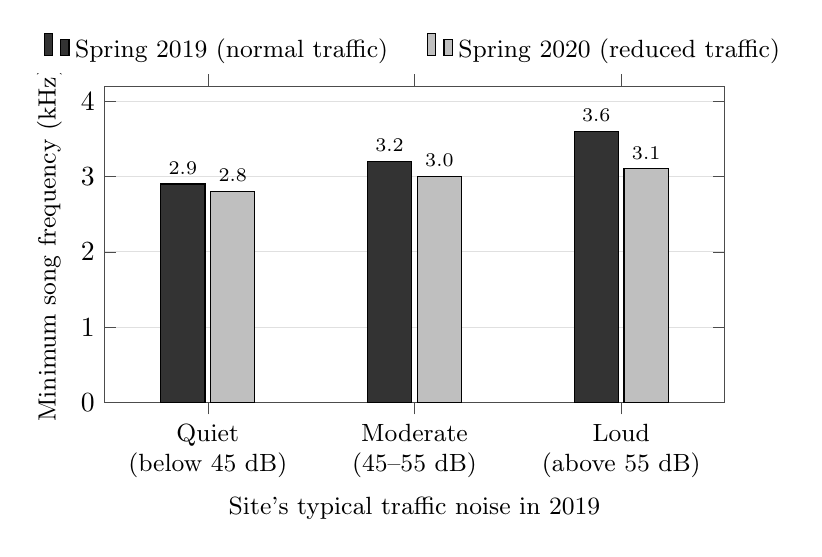
\begin{tikzpicture}
\begin{axis}[
  ybar, bar width=16pt, width=0.78\linewidth, height=5.6cm,
  ymin=0, ymax=4.2, ytick={0,1,2,3,4},
  ylabel={Minimum song frequency (kHz)}, ylabel style={font=\small},
  symbolic x coords={Quiet,Moderate,Loud},
  xticklabels={{Quiet\\(below 45 dB)},{Moderate\\(45--55 dB)},{Loud\\(above 55 dB)}},
  xticklabel style={align=center,font=\small}, xtick=data,
  xlabel={Site's typical traffic noise in 2019}, xlabel style={font=\small},
  enlarge x limits=0.25,
  nodes near coords, nodes near coords style={font=\scriptsize},
  point meta=explicit symbolic,
  legend style={at={(0.5,1.04)},anchor=south,font=\small,draw=none,legend columns=2,/tikz/every even column/.append style={column sep=12pt}},
  axis line style={black!70}, tick style={black!70},
  ymajorgrids, grid style={black!12},
]
\addplot[fill=black!80,draw=black] coordinates {(Quiet,2.9)[2.9] (Moderate,3.2)[3.2] (Loud,3.6)[3.6]};
\addplot[fill=black!25,draw=black] coordinates {(Quiet,2.8)[2.8] (Moderate,3.0)[3.0] (Loud,3.1)[3.1]};
\legend{Spring 2019 (normal traffic),Spring 2020 (reduced traffic)}
\end{axis}
\end{tikzpicture}\par\vspace{2pt}
{\small\textbf{Figure 1.} Average minimum song frequency of one songbird species at sites grouped by typical traffic noise in 2019, recorded in spring 2019 and spring 2020. Data are illustrative.}
\end{center}

\Q{KID}{D}{Central idea (R3)}{The passage explains noise-driven song changes and uses the 2020 shutdown to show how quickly birds adjust. A--C are details or absent.}
{The passage is primarily concerned with:}
{the history of noise regulation in cities.}
{why female songbirds prefer low-pitched songs.}
{methods for recording birdsong in urban areas.}
{how traffic noise affects birdsong and what a natural experiment revealed about how quickly birds respond.}

\Q{KID}{C}{Stated detail (R1)}{``concentrated at low frequencies, below about 2 kilohertz'' (\Line{p4phys}).}
{According to the passage, the sound of traffic is concentrated:}
{above about 4 kHz.}
{at the same frequencies as birds' highest notes.}
{at frequencies below about 2 kHz.}
{mainly during the spring.}

\Q{KID}{B}{Cause--effect (R4)}{``Raising the lowest notes \dots\ lifts them out of the noisiest part of the spectrum.'' A is the opposite (paragraph 6 says it may make songs \emph{less} attractive).}
{According to the passage, raising the lowest notes of a song helps a bird because it:}
{makes the song more attractive to females.}
{moves those notes out of the frequency range where traffic noise is strongest.}
{reduces the energy the bird spends singing.}
{lets the song travel farther in quiet areas.}

\Q{KID}{D}{Relationships: hypotheses (R4)}{\lines{p4p3}{p4p3end}: individual adjustment ``could occur within a single season---and should reverse when the noise goes away.'' A describes the evolutionary hypothesis.}
{According to the third paragraph, if individual birds adjust their songs in response to noise, then the change in their songs:}
{should be slow and largely fixed.}
{should appear only in young birds.}
{should make songs louder but not higher.}
{could occur within a single season and should reverse when the noise disappears.}

\Q{CS}{A}{Word choice / function (R6)}{No researcher planned the lockdowns (``unplanned''), yet they created the conditions to test the two hypotheses (``experiment''). Nothing suggests criticism (B) or unreliability (C).}
{The author describes the 2020 lockdowns as ``an unplanned experiment'' (\Line{p4exp}) primarily to indicate that:}
{traffic noise was reduced by circumstance rather than by researchers, yet the change still allowed the hypotheses to be tested.}
{researchers had failed to design their studies carefully.}
{the results of the 2020 recordings are unreliable.}
{cities should deliberately repeat the lockdowns.}

\Q{CS}{C}{Function of a paragraph (R7)}{``Singing higher solves one problem but may create another'' (\Line{p4p6}): a possible cost of the adaptation. It does not refute the study (A).}
{The sixth paragraph (\lines{p4p6}{p4p6end}) primarily serves to:}
{refute the conclusion drawn from the 2020 recordings.}
{explain how researchers measure the energy cost of singing.}
{present a possible drawback of the adaptation described earlier.}
{introduce a second species for comparison.}

\Q{IKI}{C}{Reading the figure (R11)}{Loud sites: 3.6 kHz (2019) $-$ 3.1 kHz (2020) $=$ 0.5 kHz. D is the 2020 level, not the change.}
{According to Figure 1, from spring 2019 to spring 2020, the average minimum song frequency at the loud sites changed by approximately:}
{0.1 kHz.}{0.2 kHz.}{0.5 kHz.}{3.1 kHz.}

\Q{IKI}{B}{Text--figure integration (R11)}{The loud-site bars drop 0.5 kHz, the largest change---matching ``At the noisiest sites, the drop was large'' (\Line{p4drop}). D is consistent with the passage but the figure shows song frequency, not noise levels.}
{The data in Figure 1 most directly support which statement from the passage?}
{``females appear to prefer males whose songs include lower notes''}
{``At the noisiest sites, the drop was large''}
{``singing louder and higher costs energy''}
{``traffic noise in many cities fell to levels not heard in decades''}

\Q{KID}{A}{Inference (R2)}{If birds adjust to the noise they hear, birds at quiet sites had little noise to adjust to in either year, so their songs barely changed (2.9 vs.\ 2.8 kHz). B contradicts the passage's conclusion; C and D are unsupported.}
{Based on the passage and Figure 1, the most likely reason that minimum song frequency barely changed at the quiet sites is that:}
{birds there had little traffic noise to adjust to in either year.}
{birds there had evolved lower voices over many generations.}
{researchers recorded fewer birds at the quiet sites.}
{the quiet sites were not affected by the lockdowns.}

% =====================================================================
\answerkey{%
\textbf{Scoring.} One point per correct answer. On the real test, 27 of the 36 questions are scored and the raw-to-scale conversion varies by form, so use this section to diagnose skills, not to predict an exact score.

\vspace{4pt}
\begin{center}
\small
\begin{tabular}{@{}lcccc@{}}
\toprule
\textbf{Reporting category} & \textbf{Questions} & \textbf{Share} & \textbf{Your correct} & \textbf{Your \%}\\
\midrule
Key Ideas \& Details (Rules 1--4) & \arabic{catKID} & 47\% & \rule{2.5em}{0.4pt} & \rule{2.5em}{0.4pt}\\
Craft \& Structure (Rules 5--8) & \arabic{catCS} & 31\% & \rule{2.5em}{0.4pt} & \rule{2.5em}{0.4pt}\\
Integration of Knowledge \& Ideas (Rules 9--11) & \arabic{catIKI} & 22\% & \rule{2.5em}{0.4pt} & \rule{2.5em}{0.4pt}\\
\midrule
\textbf{Total} & \arabic{qnum} & & \rule{2.5em}{0.4pt} & \rule{2.5em}{0.4pt}\\
\bottomrule
\end{tabular}
\end{center}
\vspace{2pt}
\textbf{By passage.} I Literary Narrative (1--9) \rule{2em}{0.4pt}\,/\,9 $\cdot$ II Social Science, paired (10--18) \rule{2em}{0.4pt}\,/\,9 $\cdot$ III Humanities (19--27) \rule{2em}{0.4pt}\,/\,9 $\cdot$ IV Natural Science with figure (28--36) \rule{2em}{0.4pt}\,/\,9.\par
Log every miss in the Volume~1 error log by rule and trap.}

\end{document}
